\chapter*{Introduction}

% Résumé graphique
\begin{figure}
    \centering
    %\includegraphics{}
    \caption{Une approche globale des fonctions de dommage. \textit{Dans un premier temps, les différentes formes de fonction de dommage sont représentées. Nous évaluons ensuite l'effet de choix de modélisation sur les résultats du modèle, avant de s'interroger sur les questions éthiques liées à ces choix de modélisation. Enfin, nous abordons la manière dont les produits des modèles sont utilisés dans le débat public.}}
    \label{fig:enter-label}
\end{figure}

%% Amorce

La carte et le navigateur \cite{edenhofer_mapmakers_2014}. 

Comment prendre les bonnes décisions face au changement climatique ? Si l'existence de celui-ci ainsi que l'ampleur des conséquences qu'il induit ne font plus de doute, les actions à mettre en œuvre et les choix à faire pour le limiter et s'en protéger sont moins consensuelles. Elles font l'objet de nombreux débats, aux niveaux nationaux mais aussi internationaux dans la diplomatie climatique. Un des défis de ces décisions est l'incertitude qui les entoure : on ne connait pas les conséquences de chaque décision, et pourtant, il faut choisir un chemin. Une discipline cherche à éclairer cette route sombre, à la manière des phares d'une voiture : la prospective. Un outil particulièrement utilisé pour réduire cette incertitude est la modélisation, et particulièrement la modélisation intégrée. \\

%% Définition des termes

%% Rappel du sujet

%% Problématique

%% Plan 

Le \ref{chapter:introduction} chapitre 1 est consacré à une présentation du contexte scientifique et politique dans lequel s'inscrivent les fonctions de dommage. Il présente d'abord les différents risques climatiques, c'est-à-dire les raisons pour lesquelles on s'intéresse au changement climatique. Il poursuit en présentant l'intrication entre les sciences dures et la politique dans les négociations climatiques. Enfin, il présente les outils qui permettent d'éclairer ces décisions, notamment les modèles intégrés et leurs fonctions de dommage. 

Le chapitre 2 présente la méthodologie et les résultats de la revue de littérature sur les fonctions de dommage. Il vise à présenter un état des lieux, complet mais non exhaustif, des fonctions de dommages qui sont utilisées ou non dans les modèles. Il est suivi d'une analyse de cet état des lieux, en classant les fonctions de dommages selon leur utilisation finale, leur forme ou encore les paramètres qui sont pris en compte. 

Le chapitre 3 présente l'étape de modélisation. On y réutilise les résultats de la revue de la littérature pour voir l'effet des fonctions de dommage sur le modèle WILIAM. Les différentes formes de fonctions de dommage sont introduites dans une version modifiée du modèle. En faisant varier à la fois les paramètres et les fonctions de dommages activées, on réalise de nombreux \textit{run} et on obtient ainsi un grand échantillon de résultats. On réalise alors une étude économétrique sur ces résultats, pour évaluer le pouvoir explicatif de la fonction de dommage sur les résultats du modèle. 

Le chapitre 4 propose une réflexion plus théorique sur l'éthique de la modélisation. Des exemples concrets de points de la modélisation qui incorporent des questions éthiques, comme le choix d'une fonction de dommage, la transparence et la communication des résultats, ou le choix de la valeur du taux d'actualisation, sont analysés à l'aide d'écrits sur la philosophie des sciences, notamment Jonas, Ongino et d'autres. 

Le chapitre 5 s'interroge sur la perception de ces enjeux éthiques chez les personnes qui participent au débat public sur les questions climatiques. A travers des entretiens semis-directifs chez une dizaine d'acteurs (scientifiques, techniciens, politiques et société civile), on cherche à établir quelle compréhension des enjeux éthiques transparait dans leur transposition au débat public. 

Enfin, le chapitre 6 propose une conclusion, et revient de manière synthétique et structurée sur les apports des autres chapitres. \\

Les annexes proposent des documents complémentaires, notamment un index / glossaire, qui permet de mieux situés les termes les uns par rapport aux autres. 

\begin{figure}
    \begin{center}
\begin{tikzpicture}[node distance=3.5cm, every node/.style={rectangle, draw, minimum width=2cm, minimum height=1cm}, text centered]
\node (phenomena) [rectangle, draw] {Phénomènes};
\node (representation) [rectangle, draw, right of=phenomena, text width = 2.5 cm] {Représentation \\ schématique};
\node (interpretation) [rectangle, draw, right of=representation, text width = 2.5 cm] {Interprétation};
\node (transposition) [rectangle, draw, right of=interpretation, text width = 3 cm] {Transposition \\ dans le \\ domaine réel};

\draw [->] (phenomena) -- (representation);
\draw [->] (representation) -- (interpretation);
\draw [->] (interpretation) -- (transposition);


% Ajout des images
\node (image1) [above of=phenomena, draw=none] {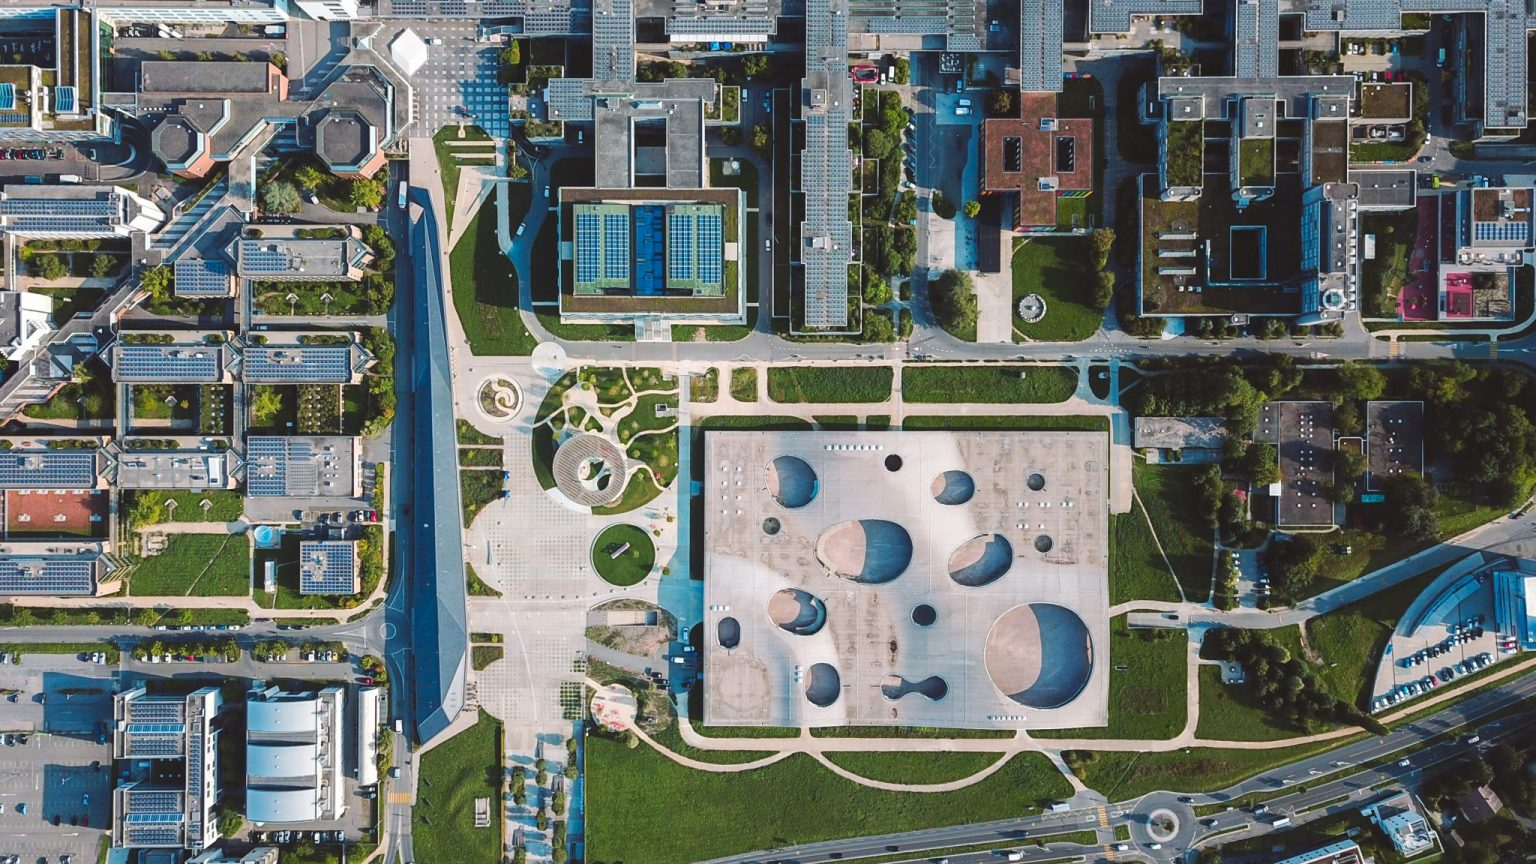
\includegraphics[width=2cm]{figures/campus.jpg}};
\node (image2) [above of=representation, draw=none, inner sep=0pt] {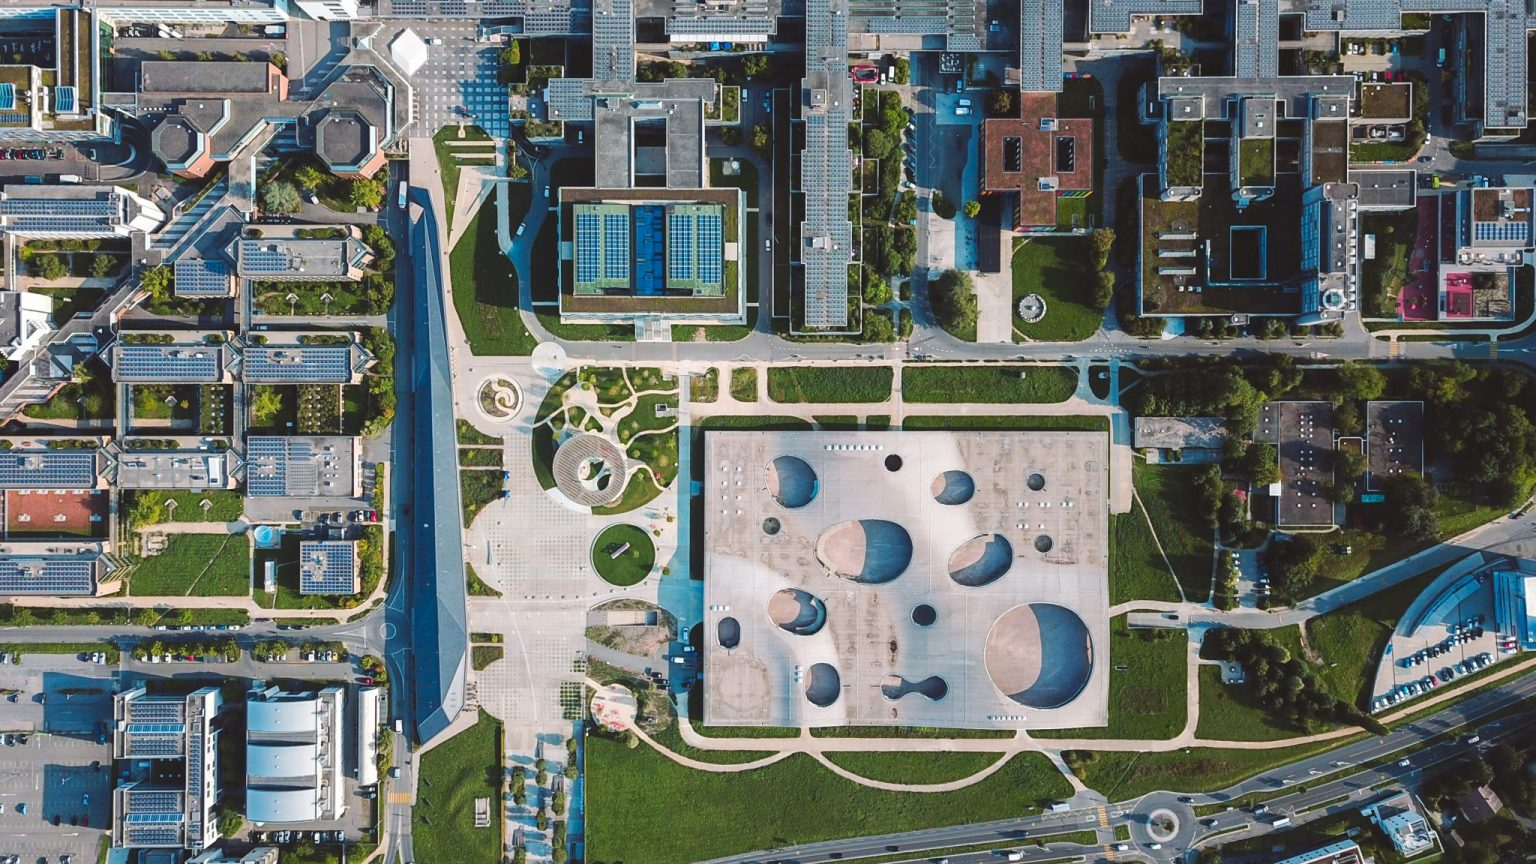
\includegraphics[width=2.5cm]{figures/campus.jpg}};
\node (image3) [above of=interpretation, inner sep=0pt] {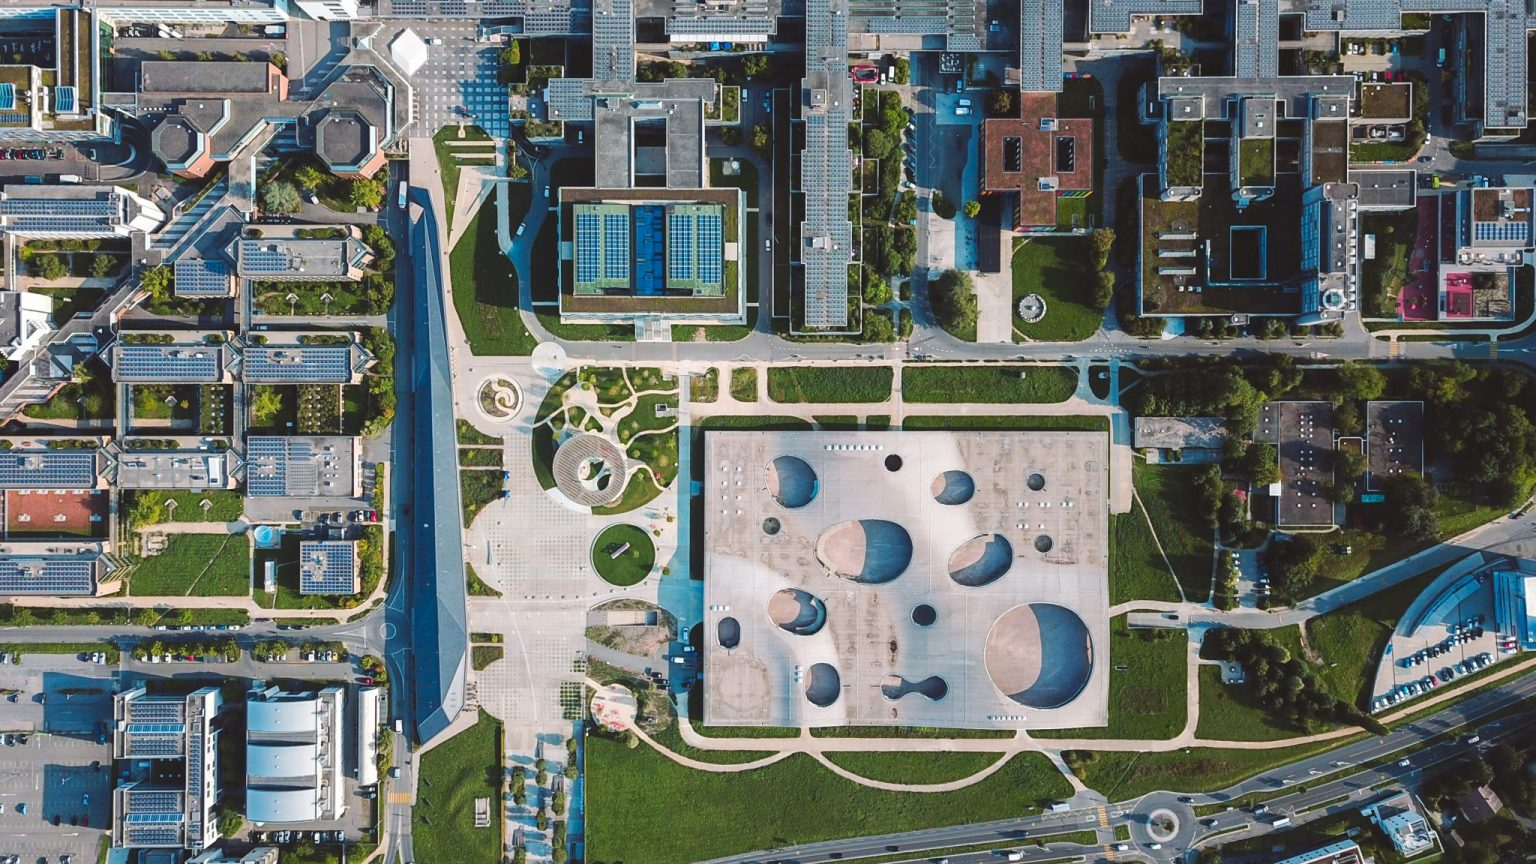
\includegraphics[width=2.5cm]{figures/campus.jpg}};
\node (image4) [above of=transposition, inner sep=0pt] {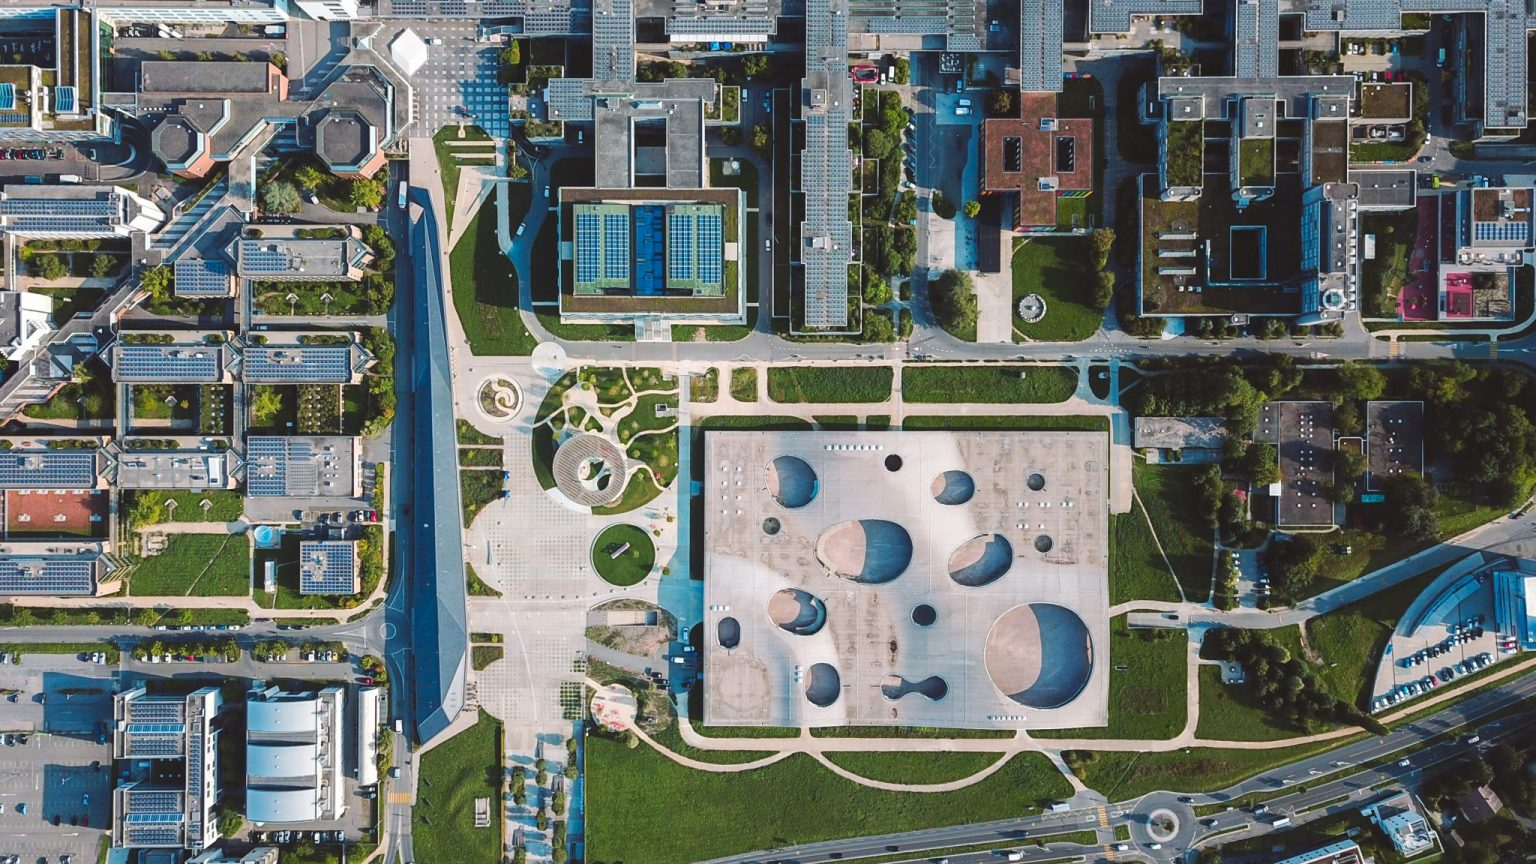
\includegraphics[width=3cm]{figures/campus.jpg}};

\end{tikzpicture}
\end{center}
    \caption{Les grandes étapes de la vie d'une modèle}
    \label{fig:enter-label}
\end{figure}